\documentclass{beamer}
\usetheme{Szeged}
\usepackage{color}
\usepackage{multirow}
\usecolortheme{dolphin}
\usefonttheme{serif}
\definecolor{light}{rgb}{0.5, 0.5, 0.5}
\def\light#1{{\color{light}#1}}

\addtobeamertemplate{navigation symbols}{}{%
    \usebeamerfont{footline}%
    \usebeamercolor[fg]{footline}%
    \hspace{1em}%
    \insertframenumber/\inserttotalframenumber
}
\title{LiDAR alapú mobil robot lokalizáció Daum–Huang-szűrő eljárással}
\author{Csuzdi Domonkos \inst{1} \and Törő Olivér \inst{2}}
\institute[KJK TDK 2021]{\inst{1} Szerző, VIK MSc. I. év \and %
                      \inst{2} Konzulens, KJIT tud. sgmts.}
\date{2021. november}
\titlegraphic{
    
\includegraphics[height=1cm]{_Figures/szechenyi2020.eps}}

\begin{document}

\frame{\titlepage}

\begin{frame}
    \frametitle{Tartalomjegyzék}
    \tableofcontents
\end{frame}
\section[Bevezetés]{Bevezetés}
\begin{frame}
    \frametitle{Motiváció}
    \begin{itemize}
        \item<1-> Daum és Huang (2008): újfajta nemlineáris szűrőeljárás: Daum--Huang-szűrő (DHF),
        majd 2010-ben: Exact Flow Daum--Huang-szűrő (EDH)
        \item<1-> Egy megoldási javaslat a részecskeszűrők problémáira
        \item<2-> Mobil robotok lokalizációja: gyakran Adaptive Monte Carlo Localization (AMCL) algoritmussal (részecskeszűrő)
        \item<2-> Egy lokalizációs probléma esetén is jobb-e az EDH?
        \item<3-> Nem vizsgáltak még EDH alapú mobil robot lokalizációt a szakirodalomban
        \item<3-> A munkám egy ilyen algoritmus kifejlesztéséről szól
    \end{itemize}

\end{frame}
\begin{frame}
    \frametitle{Lokalizáció I.}
    \begin{itemize}
        \item<1-> Egy ismert térképen követni egy objektumot (ismerni a pozíciót és orientációt)
        \item<2-> Jelen esetben csak 2D: $\mathbf{x} = [x\;\;y\;\;\theta]^{\top}$ \\
        $\to$ állapotbecslés szenzorfúzióval: pl. LiDAR és kerék enkóder
        \item<3-> Eredendően hibával terhelt mérések: sosem tudjuk pontosan a pózt
        $\to$ valószínűségi eloszlásként kezeljük
    \end{itemize}
    \begin{center}
        \includegraphics<3->[width=\linewidth]{_Figures/mcl.png}
        \only<3->{\tiny S. Thrun, W. Burgard, and D. Fox, \textit{Probabilistic robotics}. Cambridge, Mass.: MIT
            Press, 2005.}
    \end{center}
\end{frame}
\begin{frame}
    \frametitle{Lokalizáció II.}
    \begin{itemize}
        \item Bayes-féle rekurzív becslés:
              \begin{align}
                  \text{predikció:}   \nonumber                                                                                                                                                                     \\
                  \overline{bel}(\mathbf{x}_t) & = \int \underbrace{p(\mathbf{x}_t | \mathbf{x}_{t-1},\mathbf{u}_t)}_{\text{mozgásmodell}}bel(\mathbf{x}_{t-1})\mathrm{d}\mathbf{x}_{t-1}, \label{eq:bayes-predict} \\
                  \text{korrekció:}  \nonumber                                                                                                                                                                      \\
                  bel(\mathbf{x}_t)            & = \eta \underbrace{p(\mathbf{\mathbf{z}}_t | \mathbf{x}_t)}_{\text{szenzormodell}}\overline{bel}(\mathbf{x}_t).
              \end{align}
    \end{itemize}
\end{frame}
\section{Szenzormodell}
\begin{frame}
    \frametitle{Módszerek}
    \begin{columns}[t]
        \begin{column}<1->{0.5\textwidth}
            \begin{block}{Hagyományos modell}
                \hspace{1cm}
                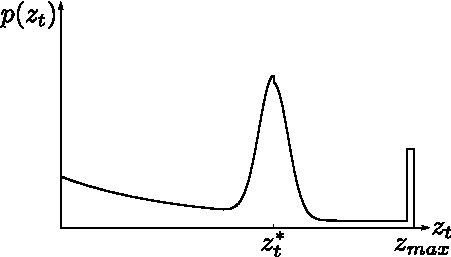
\includegraphics[width=\linewidth]{_Figures/beam-model.pdf}
                \begin{itemize}
                    \item Pásztázó távolságmérőkhöz
                    \item Nem folytonos: \\
                          $\to$ részecskeszűrőhöz (AMCL) jó, EDH-hoz nem
                \end{itemize}
            \end{block}
        \end{column}
        \begin{column}<2->{0.5\textwidth}
            \begin{block}{Távolság-transzformáció alapú modell}
                \begin{itemize}
                    \item Dantanarayana és mtsai. 2016-ban
                    \item Eredetileg EKF-hez
                    \item Foglaltsági hálón alapuló térkép + pásztázó távolságmérő (pl. LiDAR)
                    \item Alapgondolat: távolság-transzformáció (képfeldolgozás)
                \end{itemize}
            \end{block}
        \end{column}
    \end{columns}
\end{frame}

\begin{frame}
    \frametitle{Távolság-transzformáció alapú mérési modell I.}
    \begin{itemize}[<+->]
        \item Távolság transzformáció: átlagos eltérés mérhető két ponthalmaz között
        \item Két ponthalmaz: foglalt cellák a térképen és a LiDAR sugarak ,,végpontjai''
        \item Eltérés számítása (skalár): $\psi(\mathbf{x},\mathbf{z},\mathbf{m})$
        \item Ideális eset (minden végpont foglalt cellán): $\psi(\mathbf{x},\mathbf{z},\mathbf{m}) = 0$
        \item $\psi$ deriváltjai már számíthatóak: megfelel az Exact Flow Daum--Huang (EDH) szűrőhöz
        \item \textbf{Az EDH-t módosítani kellett, hogy kezeljen implicit mérési egyenletet} (eredetileg $\mathbf{z} = h(\mathbf{x})$ alak)
    \end{itemize}
\end{frame}
\section[Daum--Huang-szűrő]{Daum--Huang-szűrő}
\begin{frame}
    \frametitle{Daum--Huang-szűrő (DHF)}
    \begin{itemize}
        \item<1-> Korrigálás (priorból poszteriorba)
        \begin{itemize}
            \item részecskeszűrő: újramintavételezés (egyfajta ,,ugrás'')
            \item DHF: ,,ugrás'' helyett \textbf{részecskefolyam}
        \end{itemize}
        \item<2-> Folytonos átmenet (homotópia) priorból poszteriorba:
        \begin{equation}\label{eq:bayes-loghom}
            \log p(\mathbf{x},\lambda) = \log \underbrace{g(\mathbf{x})}_{\text{\tiny{prior}}} + \lambda \log \underbrace{h(\mathbf{x})}_{\text{\tiny{szenzormodell}}} - \log \underbrace{K(\lambda)}_{\text{\tiny{norm. konstans}}}. \nonumber
        \end{equation}
        \item<2-> $\lambda = 0$: prior, $\lambda = 1$: poszterior
        \item<3-> Részecskék mozgását egy SDE írja le ($\lambda$: pszeudoidő):
        \begin{equation}
            \mathrm{d} \mathbf{x}_i=\mathbf{f}(\mathbf{x}_i, \lambda) \mathrm{d} \lambda+\boldsymbol{\sigma}(\mathbf{x}_i, \lambda) \mathrm{d} \mathbf{W}_{\lambda},
        \end{equation}
        \item<4-> Kérdés: mi $\mathbf{f}$, (mi $\boldsymbol{\sigma}$)?
        \item<4-> Különböző Daum--Huang-szűrő variációk más-más megoldást adnak.
    \end{itemize}
\end{frame}
\begin{frame}
    \frametitle{Exact Flow Daum--Huang-szűrő (EDH)}
    \begin{itemize}[<+->]
        \item Hanyagoljuk el a sztochasztikus részt, így \\
              \begin{equation}\label{eq:ode}
                  \frac{\mathrm{d}\mathbf{x}_i}{\mathrm{d}\lambda} = \mathbf{f}(\mathbf{x}_i,\lambda).
              \end{equation}
        \item Legyen $\mathbf{f}$ alakja
              \begin{equation}\label{eq:edh-flow-vector}
                  \mathbf{f}(\mathbf{x}_i,\lambda) = \mathbf{C}(\lambda)\mathbf{x}_i + \mathbf{c}(\lambda).
              \end{equation}
        \item Együtthatók meghatározása:
              \begin{align}
                   & \light{\mathbf{C}(\lambda) = -\frac{1}{2}\mathbf{\mathbf{\overline\Sigma}}\nabla \psi_x^\top\left(\lambda \nabla \psi_x\mathbf{\overline\Sigma}\nabla \psi_x^\top + \mathbf{R}\right)^{-1}\nabla \psi_x,\label{eq:edh-C}     }                          \\
                   & \light{\mathbf{c}(\lambda) = \left(\mathbf{I}+2\lambda\mathbf{C}\right)\left[\left(\mathbf{I}+\lambda\mathbf{C}\right)\mathbf{\overline\Sigma}\nabla \psi_x^\top\mathbf{R}^{-1}\mathbf{z}' + \mathbf{C}\overline{\mathbf{x}}\right]. } \label{eq:edh-c}
              \end{align}
        \item Innentől adott a részecskék mozgása: Euler integrálása \eqref{eq:ode}-nek
    \end{itemize}
\end{frame}
\begin{frame}{EDH: részecskék mozgása}
    \begin{overlayarea}{\textwidth}{\textheight}
        \begin{figure}
            \centering
            \only<1>
            {%
                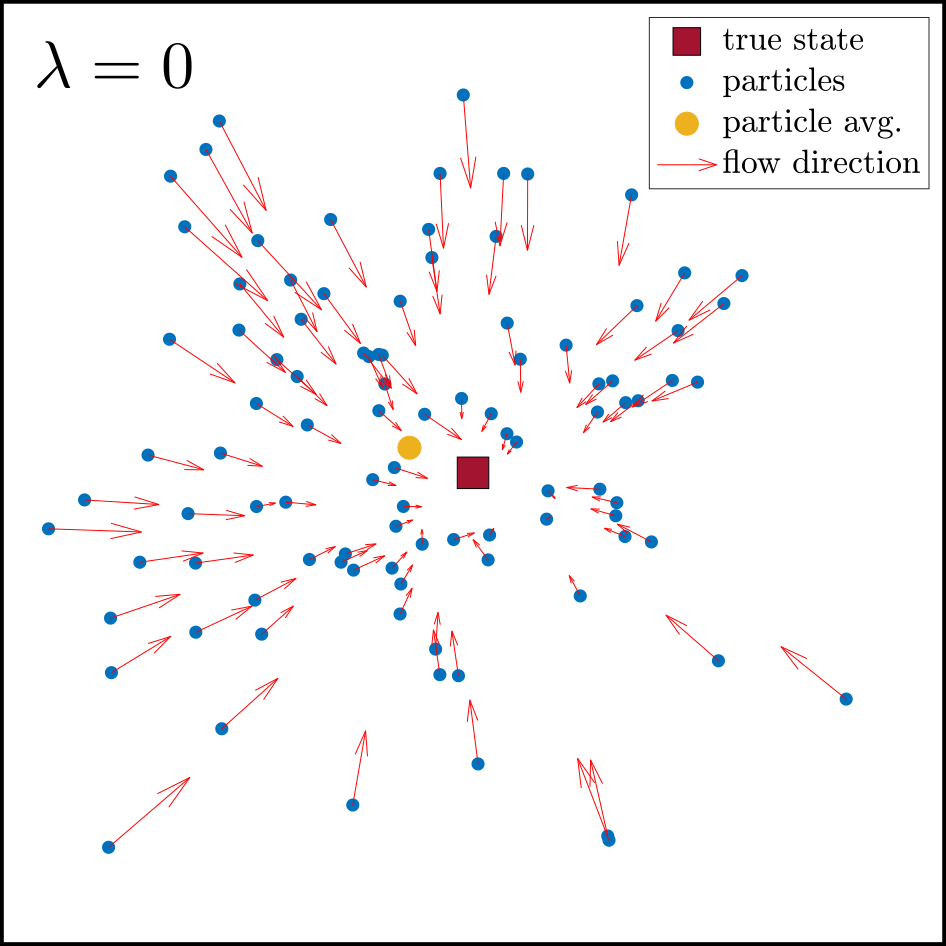
\includegraphics[width=.6\textwidth]{_Figures/l0.png}%
            }%
            \only<2>
            {%
                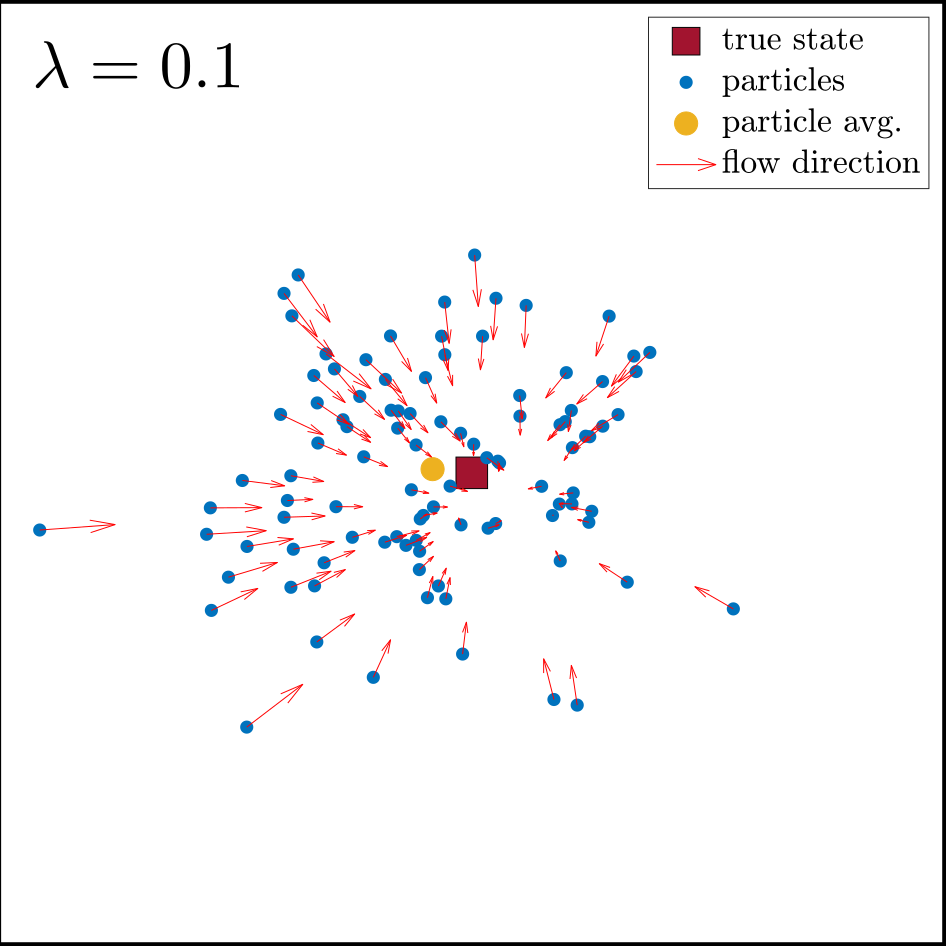
\includegraphics[width=.6\textwidth]{_Figures/l01.png}%
            }%
            \only<3>
            {%
                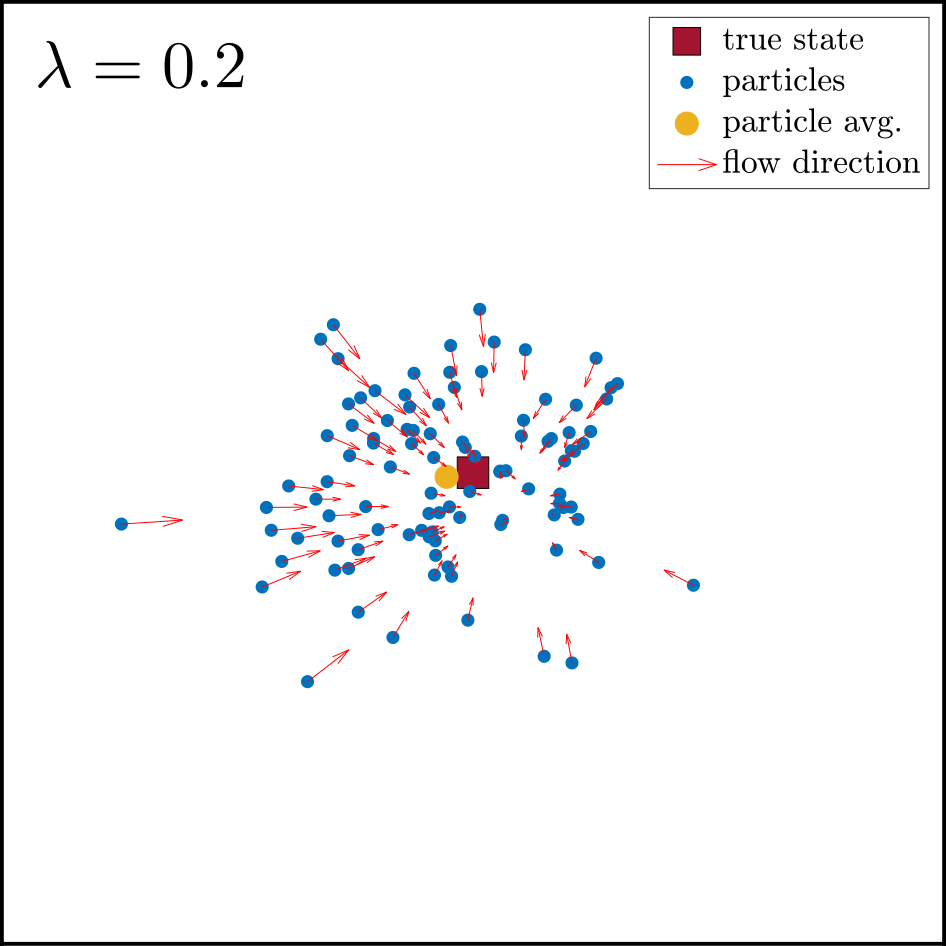
\includegraphics[width=.6\textwidth]{_Figures/l02.png}%
            }%
            \only<4>
            {%
                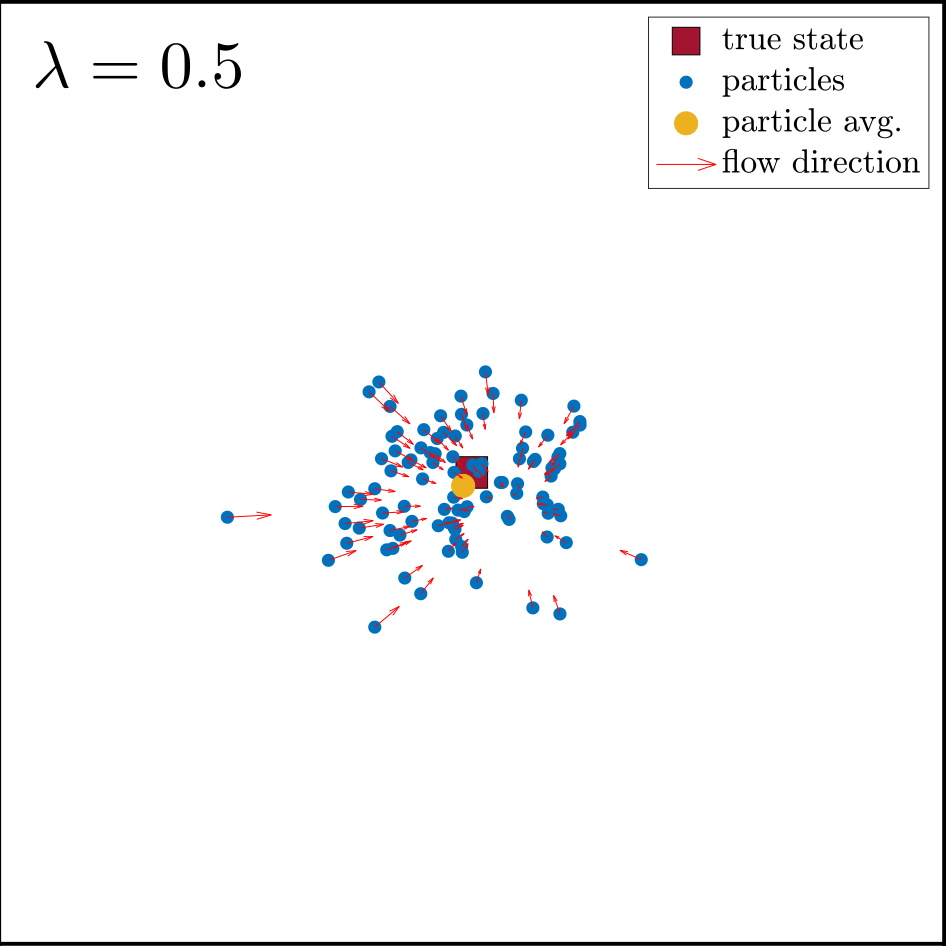
\includegraphics[width=.6\textwidth]{_Figures/l05.png}%
            }%
            \only<5>
            {%
                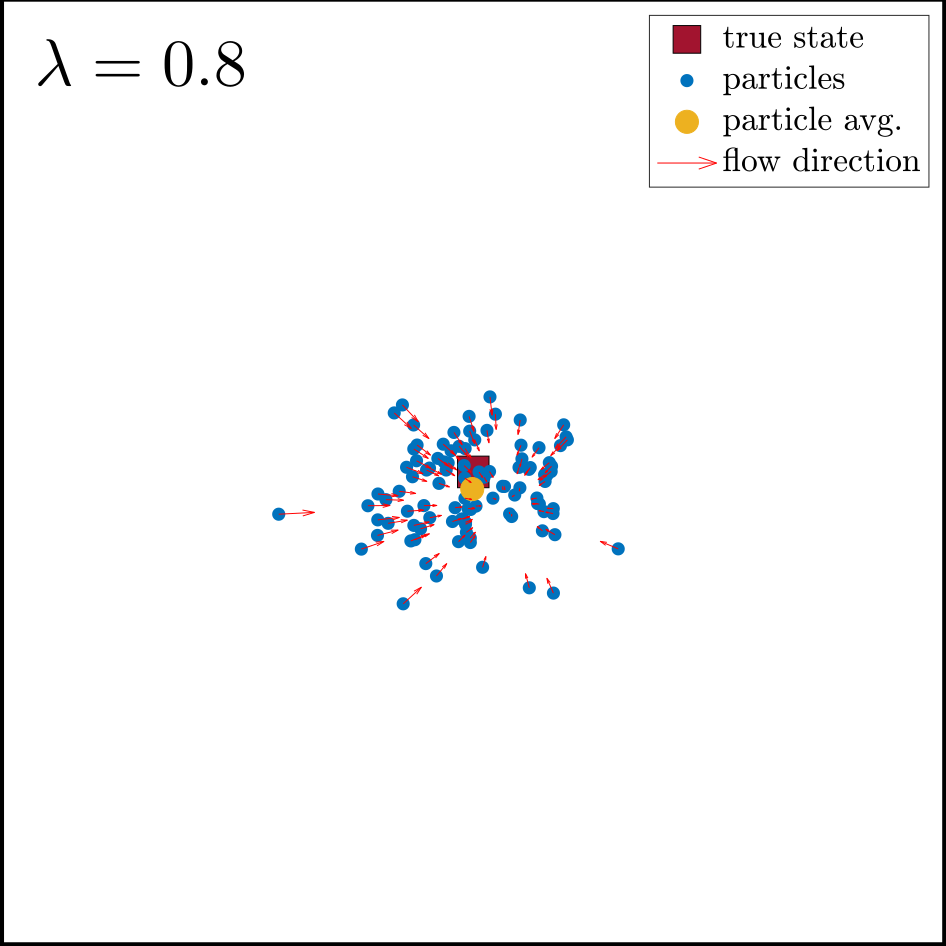
\includegraphics[width=.6\textwidth]{_Figures/l08.png}%
            }%
            \only<6>
            {%
                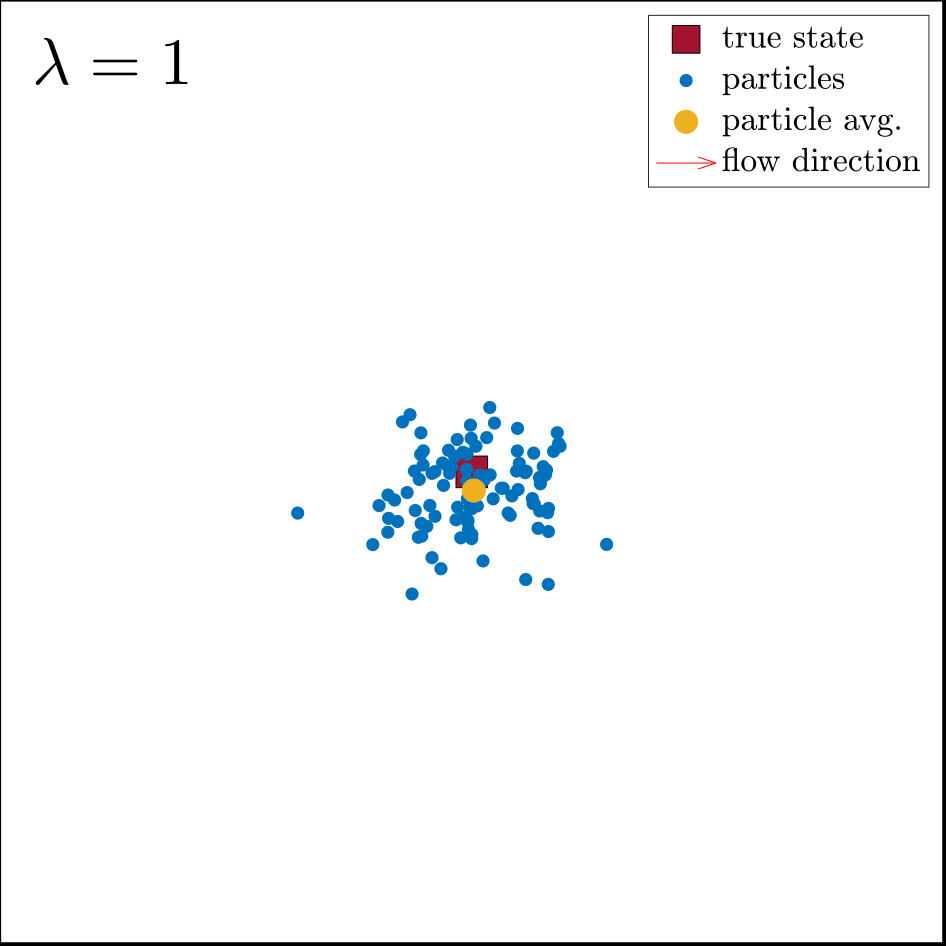
\includegraphics[width=.6\textwidth]{_Figures/l1.png}%
            }%
        \end{figure}
    \end{overlayarea}

\end{frame}
\section{Eredmények}
\begin{frame}
    \frametitle{Tesztelési összeállítás}
    \begin{columns}
        \begin{column}{0.65\textwidth}
            \begin{itemize}
                \item<1-> ROBOTIS Turtlebot3 Burger
                \item<1-> Gazebo szimulátor + Robot Operating System (ROS)
                \item<2-> Környezet: Turtlebot3 House
                \item<3-> Kb. 7-8 percnyi barangolás (manuálisan)
                \item<4-> Valós póz és becsült póz összehasonlítása
                \item<5-> Algoritmusok: AMCL, és a készített EDH alapú
            \end{itemize}
        \end{column}
        \begin{column}{0.5\textwidth}
            \begin{center}
                \vspace{-1.5cm}
                \includegraphics<1->[width=0.8\linewidth]{_Figures/turtlebot3.pdf}
                \includegraphics<2->[width=\linewidth]{_Figures/tb3_house.png}
            \end{center}
        \end{column}
    \end{columns}
\end{frame}
\begin{frame}
    \frametitle{AMCL eredmény}
    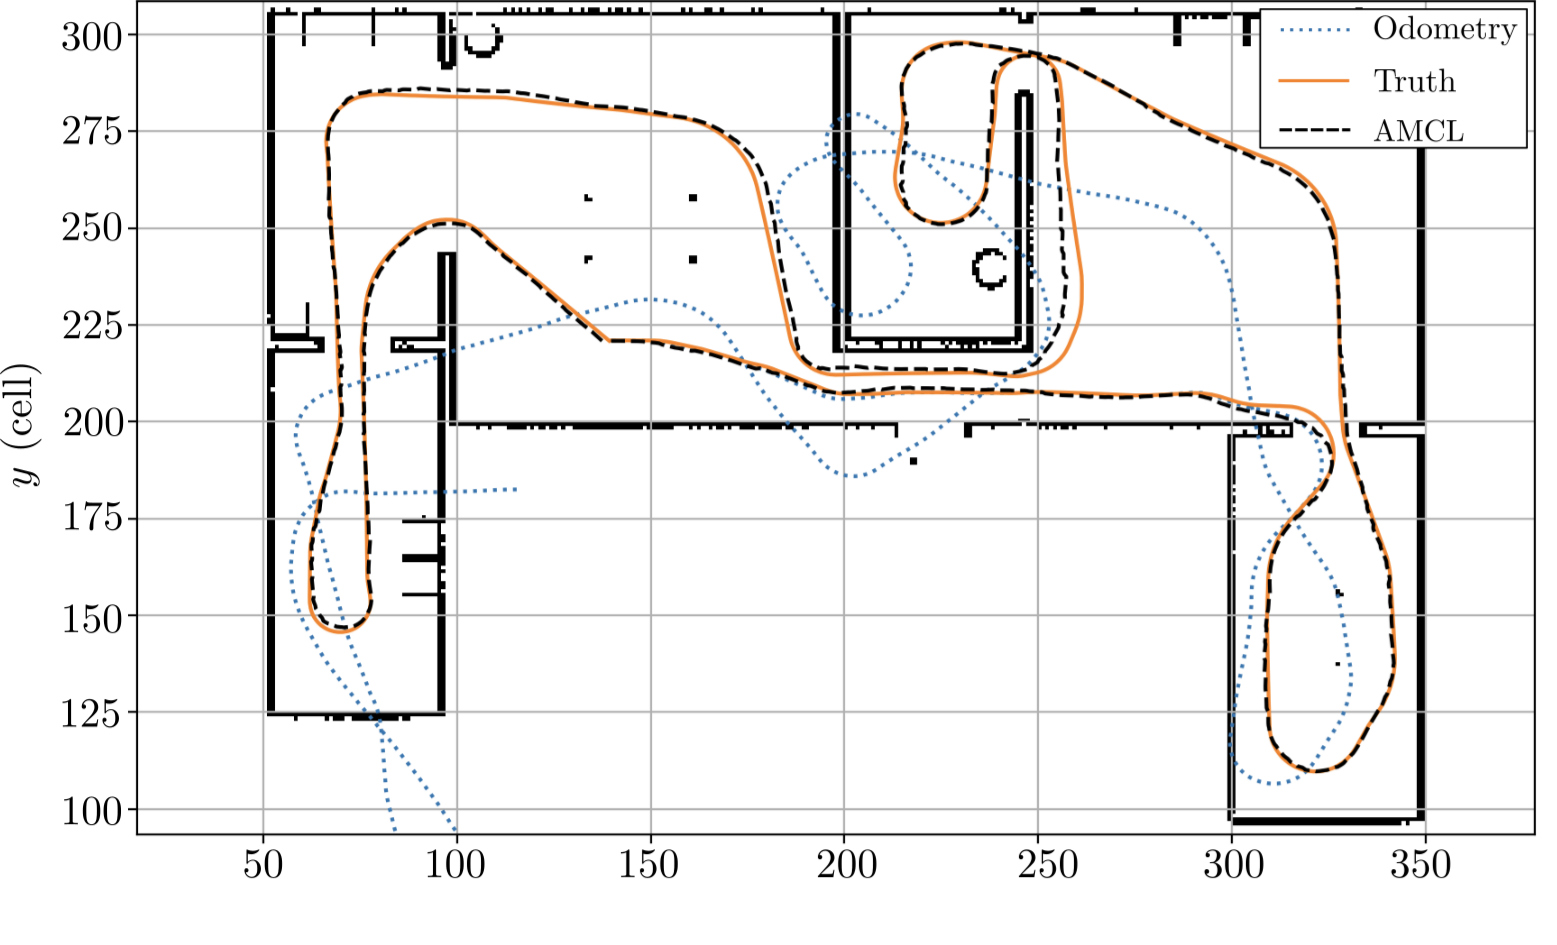
\includegraphics[width=\linewidth]{_Figures/AMCL_crop.png}
\end{frame}
\begin{frame}
    \frametitle{EDH eredmény}
    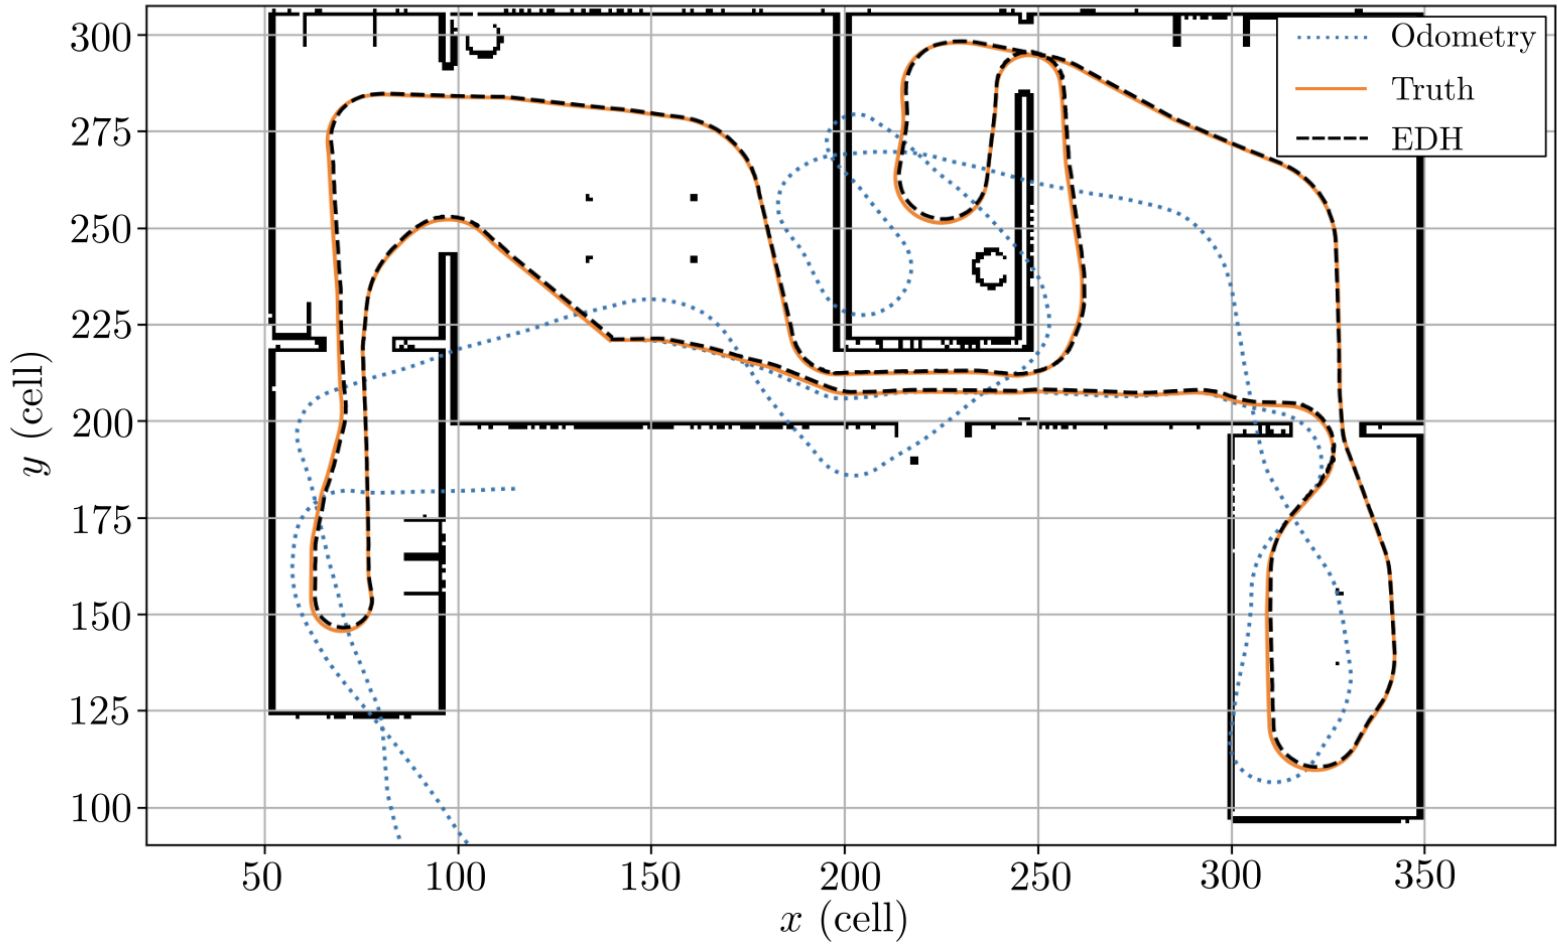
\includegraphics[width=\linewidth]{_Figures/EDH_crop.png}
\end{frame}
\begin{frame}
    \frametitle{Pozíció hiba ($x$ irány)}
    \begin{center}
        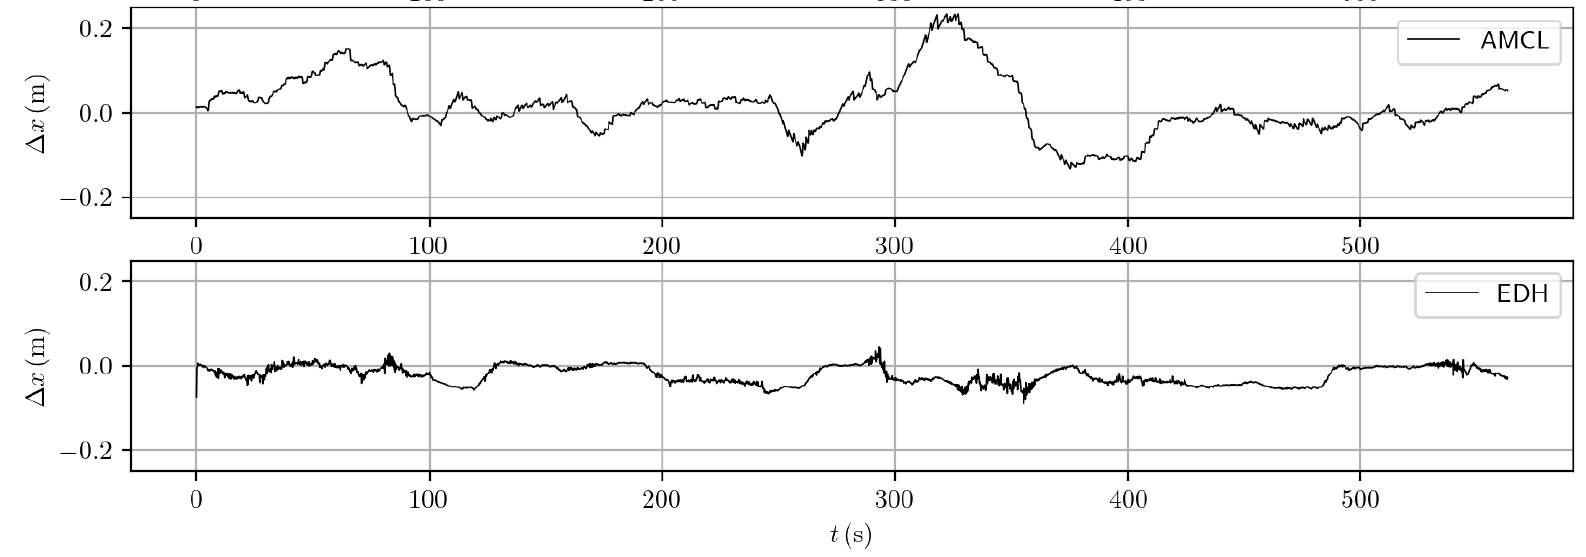
\includegraphics[width=1\linewidth]{_Figures/dx.png}
    \end{center}
    \tiny\begin{table}[]
        \centering
        \begin{tabular}{lllllll}
            \hline
            \multicolumn{1}{|c|}{\multirow{2}{*}{Algoritmus}} & \multicolumn{1}{c|}{\multirow{2}{*}{\begin{tabular}[c]{@{}c@{}}$\kappa$\\(m)\end{tabular}}} & \multicolumn{1}{c|}{\multirow{2}{*}{\begin{tabular}[c]{@{}c@{}}Részecske\\szám\end{tabular}}} & \multicolumn{2}{c|}{Root Mean Squared Error}    & \multicolumn{2}{c|}{Mean Absolute Error}                                                                                                            \\\cline{4-7}
            \multicolumn{1}{|c|}{}                            & \multicolumn{1}{c|}{}                                            & \multicolumn{1}{c|}{}                                            & \multicolumn{1}{l|}{\begin{tabular}[c]{@{}c@{}}pozíció\\ (m)\end{tabular}} & \multicolumn{1}{c|}{\begin{tabular}[c]{@{}c@{}}orientáció\\ (rad)\end{tabular}} & \multicolumn{1}{l|}{\begin{tabular}[c]{@{}c@{}}pozíció\\ ($\text{m}$)\end{tabular}} & \multicolumn{1}{l|}{\begin{tabular}[c]{@{}c@{}}orientáció\\ ($\text{rad}$)\end{tabular}} \\ \hline
            \hline
            \multicolumn{1}{|l|}{AMCL}                        & \multicolumn{1}{c|}{$10^{-4}$}                                   & \multicolumn{1}{c|}{adaptív}                                     & \multicolumn{1}{c|}{0.0816}                     & \multicolumn{1}{c|}{0.0708}                     & \multicolumn{1}{c|}{0.0672}                     & \multicolumn{1}{c|}{0.0547}                     \\ \hline
            \multicolumn{1}{|l|}{\multirow{3}{*}{EDH}}        & \multicolumn{1}{c|}{\multirow{3}{*}{$10^{-4}$}}                  & \multicolumn{1}{c|}{10}                                          & \multicolumn{1}{c|}{0.0439}                     & \multicolumn{1}{c|}{0.0205}                     & \multicolumn{1}{c|}{\textbf{0.0381}}            & \multicolumn{1}{c|}{0.0188}                     \\ \cline{3-7}
            \multicolumn{1}{|l|}{}                            & \multicolumn{1}{c|}{}                                            & \multicolumn{1}{c|}{100}                                         & \multicolumn{1}{c|}{\textbf{0.0437}}            & \multicolumn{1}{c|}{0.0206}                     & \multicolumn{1}{c|}{0.0383}                     & \multicolumn{1}{c|}{0.0190}                     \\ \cline{3-7}
            \multicolumn{1}{|l|}{}                            & \multicolumn{1}{c|}{}                                            & \multicolumn{1}{c|}{500}                                         & \multicolumn{1}{c|}{0.0438}                     & \multicolumn{1}{c|}{0.0206}                     & \multicolumn{1}{c|}{0.0382}                     & \multicolumn{1}{c|}{0.0190}                     \\ \hline
        \end{tabular}
    \end{table}



\end{frame}
\begin{frame}
    \frametitle{Orientáció hiba}
    \begin{center}
        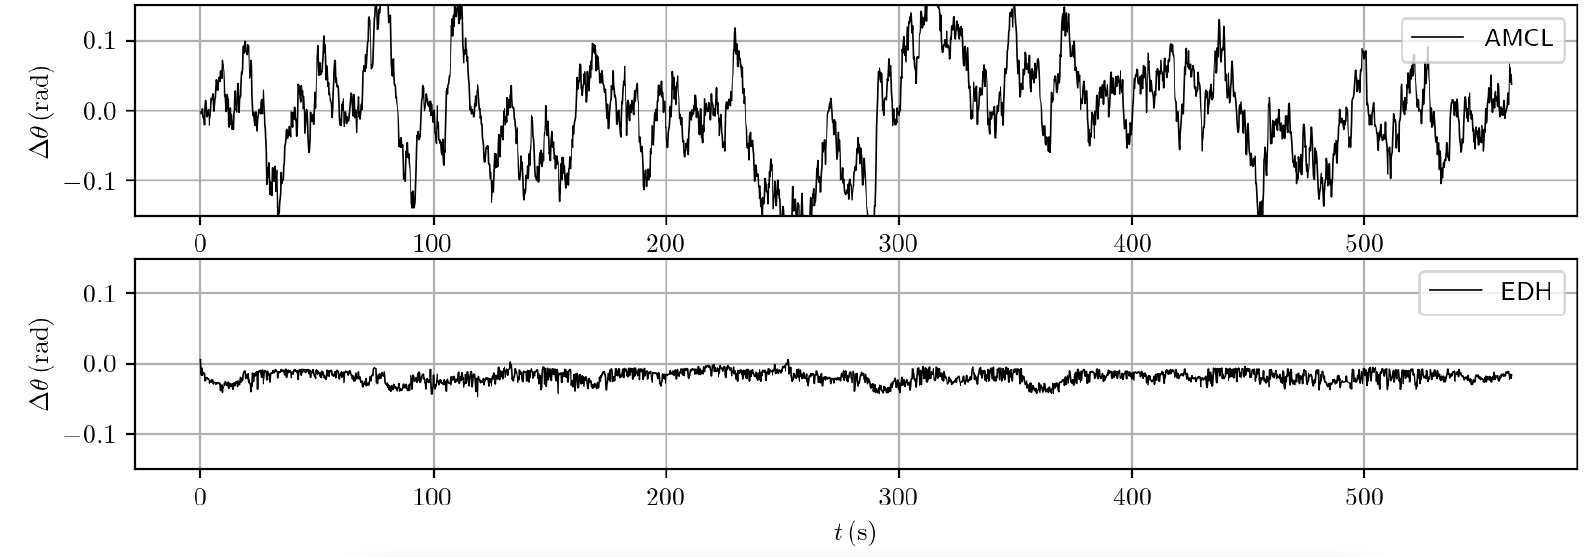
\includegraphics[width=1\linewidth]{_Figures/dfi.png}
    \end{center}
    \tiny\begin{table}[]
        \centering
        \begin{tabular}{lllllll}
            \hline
            \multicolumn{1}{|c|}{\multirow{2}{*}{Algoritmus}} & \multicolumn{1}{c|}{\multirow{2}{*}{\begin{tabular}[c]{@{}c@{}}$\kappa$\\(m)\end{tabular}}} & \multicolumn{1}{c|}{\multirow{2}{*}{\begin{tabular}[c]{@{}c@{}}Részecske\\szám\end{tabular}}} & \multicolumn{2}{c|}{Root Mean Squared Error}    & \multicolumn{2}{c|}{Mean Absolute Error}                                                                                                            \\\cline{4-7}
            \multicolumn{1}{|c|}{}                            & \multicolumn{1}{c|}{}                                            & \multicolumn{1}{c|}{}                                            & \multicolumn{1}{l|}{\begin{tabular}[c]{@{}c@{}}pozíció\\ (m)\end{tabular}} & \multicolumn{1}{c|}{\begin{tabular}[c]{@{}c@{}}orientáció\\ (rad)\end{tabular}} & \multicolumn{1}{l|}{\begin{tabular}[c]{@{}c@{}}pozíció\\ ($\text{m}$)\end{tabular}} & \multicolumn{1}{l|}{\begin{tabular}[c]{@{}c@{}}orientáció\\ ($\text{rad}$)\end{tabular}} \\ \hline
            \hline
            \multicolumn{1}{|l|}{AMCL}                        & \multicolumn{1}{c|}{$10^{-4}$}                                   & \multicolumn{1}{c|}{adaptív}                                     & \multicolumn{1}{c|}{0.0816}                     & \multicolumn{1}{c|}{0.0708}                     & \multicolumn{1}{c|}{0.0672}                     & \multicolumn{1}{c|}{0.0547}                     \\ \hline
            \multicolumn{1}{|l|}{\multirow{3}{*}{EDH}}        & \multicolumn{1}{c|}{\multirow{3}{*}{$10^{-4}$}}                  & \multicolumn{1}{c|}{10}                                          & \multicolumn{1}{c|}{0.0439}                     & \multicolumn{1}{c|}{\textbf{0.0205}}            & \multicolumn{1}{c|}{0.0381}                     & \multicolumn{1}{c|}{\textbf{0.0188}}            \\ \cline{3-7}
            \multicolumn{1}{|l|}{}                            & \multicolumn{1}{c|}{}                                            & \multicolumn{1}{c|}{100}                                         & \multicolumn{1}{c|}{0.0437}                     & \multicolumn{1}{c|}{0.0206}                     & \multicolumn{1}{c|}{0.0383}                     & \multicolumn{1}{c|}{0.0190}                     \\ \cline{3-7}
            \multicolumn{1}{|l|}{}                            & \multicolumn{1}{c|}{}                                            & \multicolumn{1}{c|}{500}                                         & \multicolumn{1}{c|}{0.0438}                     & \multicolumn{1}{c|}{0.0206}                     & \multicolumn{1}{c|}{0.0382}                     & \multicolumn{1}{c|}{0.0190}                     \\ \hline
        \end{tabular}
    \end{table}
\end{frame}
\section{Összegzés}
\begin{frame}
    \frametitle{Összegzés}
    \begin{itemize}
        \item<1-> Magabiztosan jobb eredmények, mint az AMCL esetén
        \item<1-> Képes valós idejű futásra:  439 s-nyi mérési adatra 40.4 s
        \item<2-> Jövőben:
        \begin{itemize}
            \item Robusztusság tesztelése (pl. ,,elrabolt robot'' probléma)
            \item Egyéb DHF variációk (pl. sztochasztikus rész)
            \item Futásidő csökkentése
            \item Futtatás valós mérési adatokon
            \item Az eredmények publikálása
        \end{itemize}
    \end{itemize}
\end{frame}
\begin{frame}{}
    \centering \Huge
    {Köszönöm a figyelmet!}
\end{frame}
\appendix
\section{Kiegészítés}
\begin{frame}
    \frametitle{LiDAR mérések projekciója}
    \begin{center}
        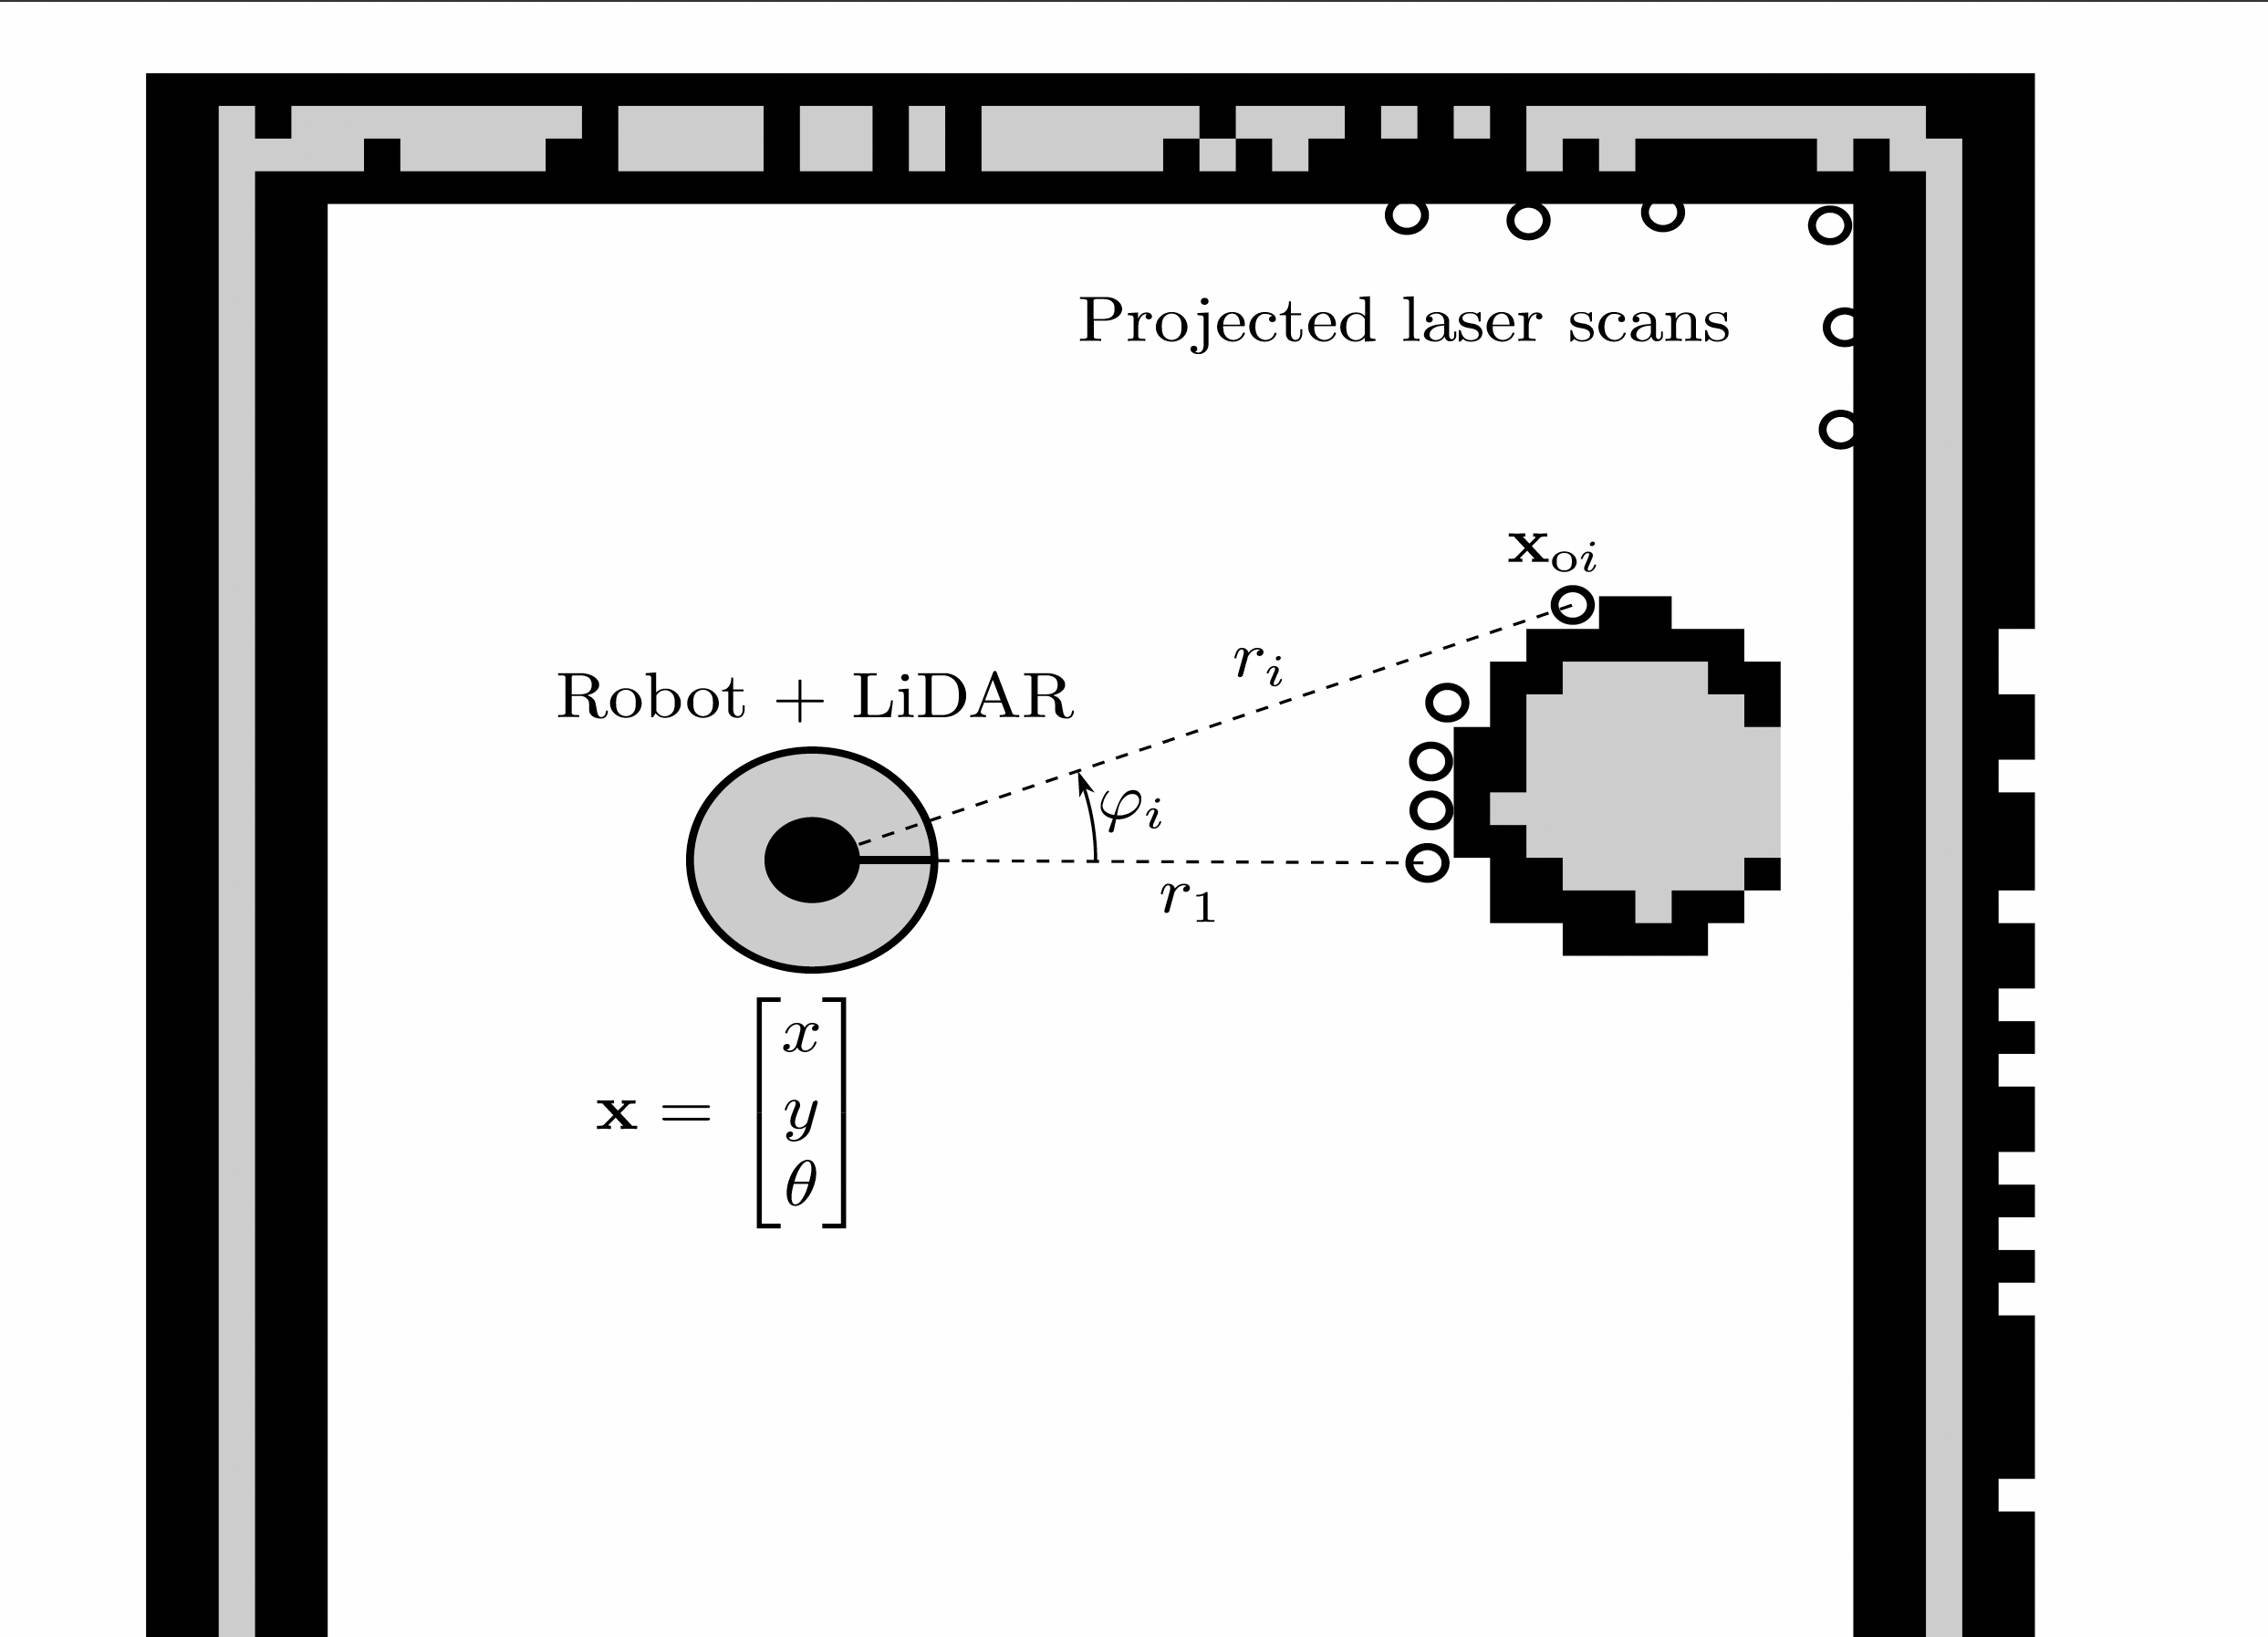
\includegraphics[width=0.8\linewidth]{_Figures/dt_mapping_lidar.png}
    \end{center}
\end{frame}
\begin{frame}
    \frametitle{Részecske degeneráció}
    \begin{center}
        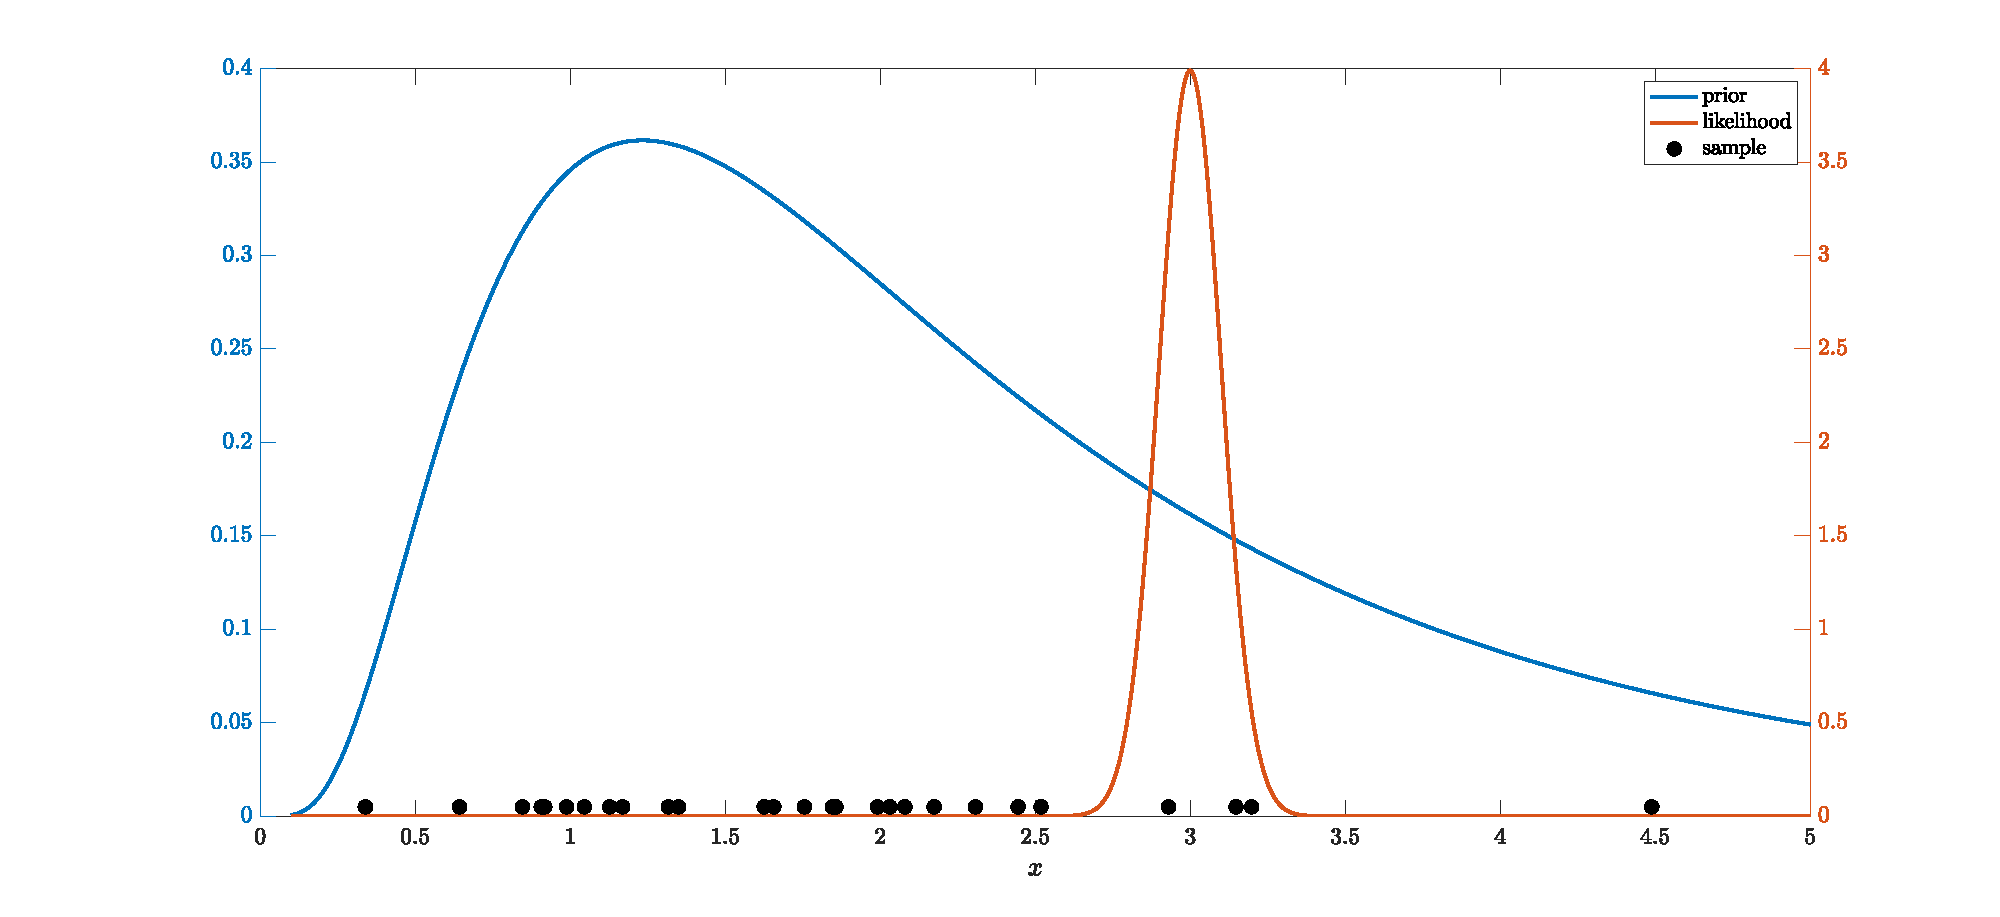
\includegraphics[width=1\linewidth]{_Figures/pf_degen.pdf}
    \end{center}
\end{frame}
\begin{frame}
    \frametitle{Részletes eredmények}
    \begin{center}
        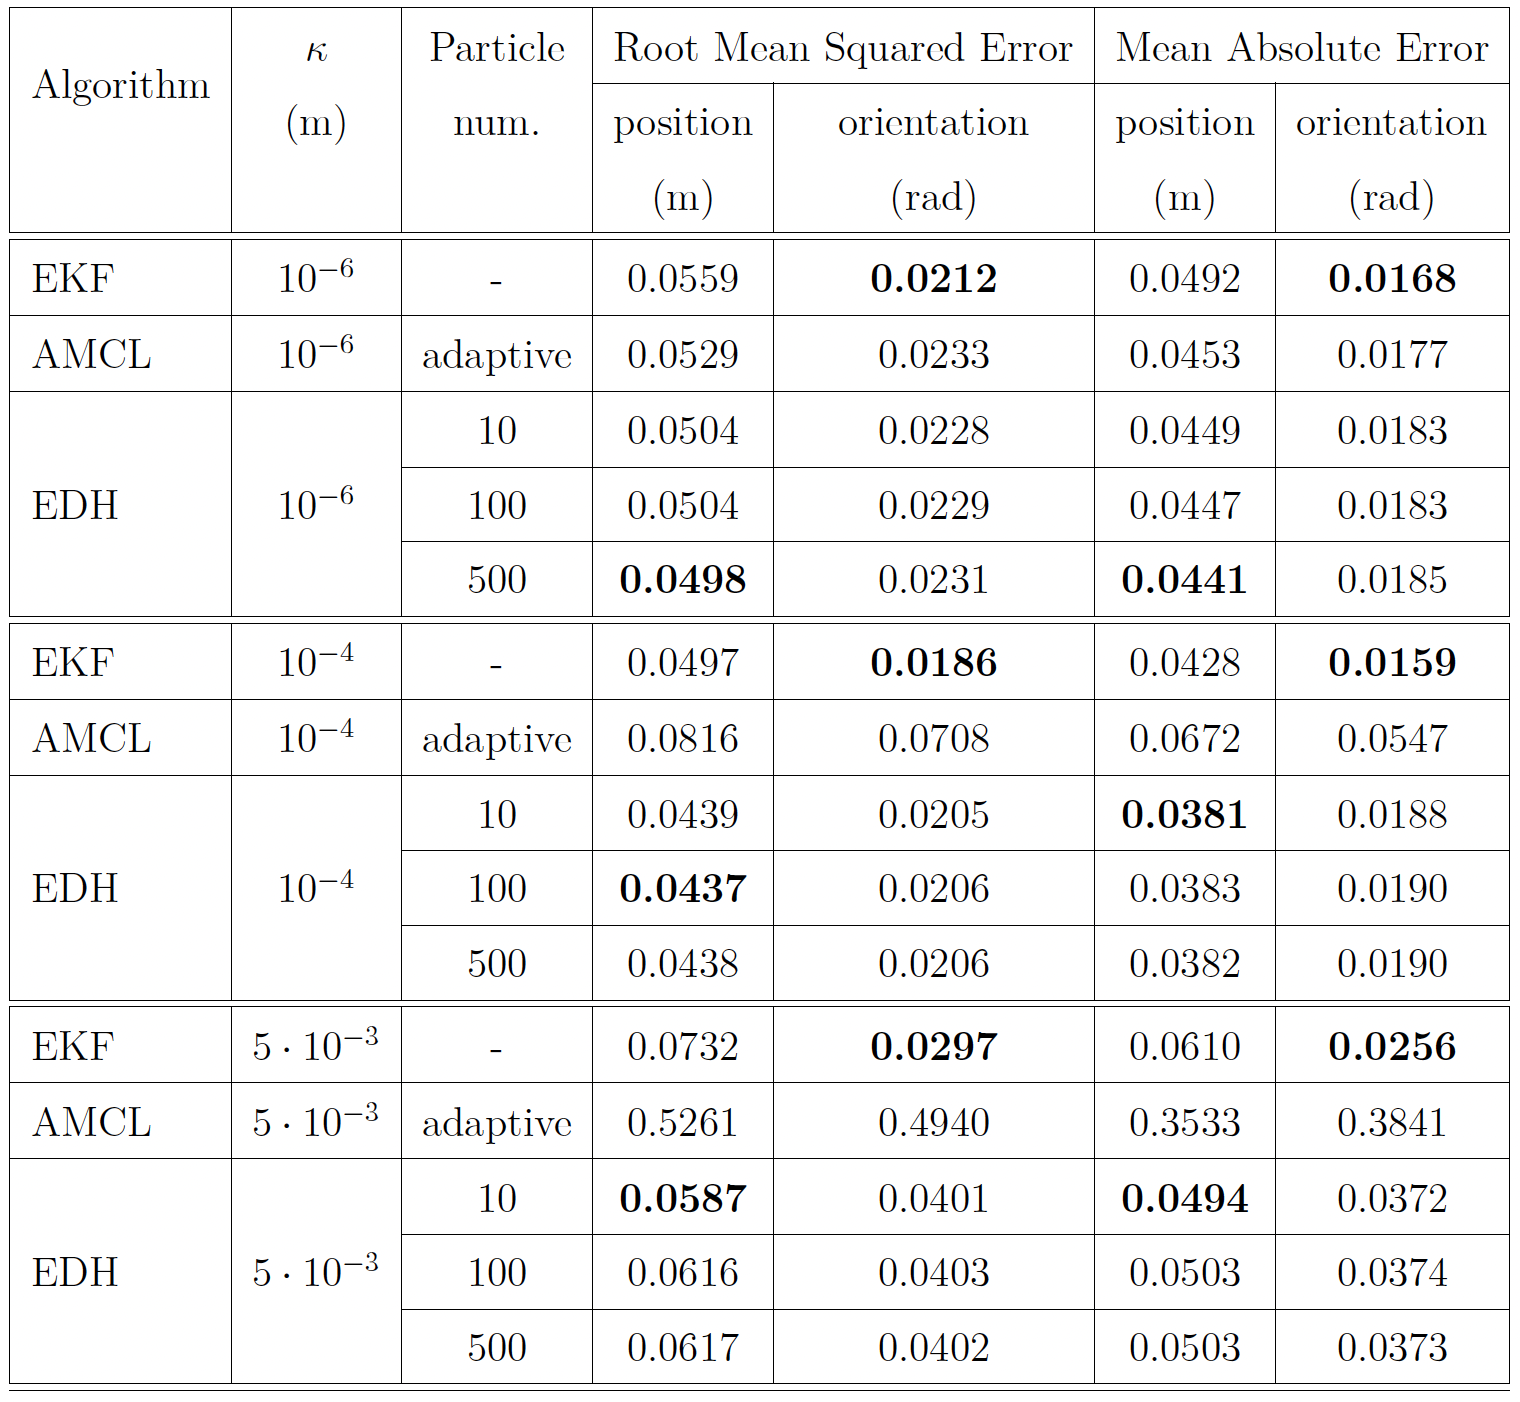
\includegraphics[width=0.7\linewidth]{_Figures/results_table.png}
    \end{center}
\end{frame}
\begin{frame}
    \frametitle{Távolság-transzformáció alapú mérési modell (kieg.)}
    \begin{columns}[t]
        \begin{column}[]{0.3\textwidth}
            \begin{center}
                \vspace{-1cm}
                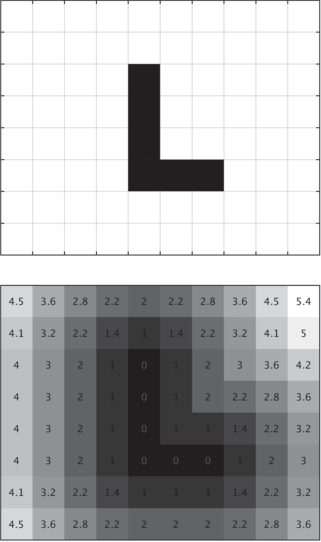
\includegraphics[width=1.2\linewidth]{_Figures/simple_dt_vertical.pdf}
            \end{center}
        \end{column}
        \begin{column}[]{0.7\textwidth}
            \begin{equation}
                D F(\mathbf{x},\mathbf{m})=\min _{\mathbf{v}_{\mathbf{j}} \in V}\left\|\mathbf{x}-\mathbf{v}_{\mathbf{j}}\right\|,
            \end{equation}
            \begin{equation}\label{eq:ray-projection}
                \mathbf{x}_{\mathrm{o}i} = \begin{bmatrix}x_{\mathrm{o}i}\\y_{\mathrm{o}i}\end{bmatrix}
                = \begin{bmatrix}x + r_i\cos(\varphi_i + \theta)\\y + r_i\sin(\varphi_i + \theta)\end{bmatrix},
            \end{equation}
            \begin{equation}
                \psi(\mathbf{x},\mathbf{z},\mathbf{m}) = \frac{1}{n}\sum_{i=1}^nDF(\mathbf{x}_{\text{o}i},\mathbf{m}).
            \end{equation}
        \end{column}
    \end{columns}
\end{frame}
\end{document}
